\documentclass[hyperref={colorlinks = true},unknownkeysallowed]{beamer}
\usepackage{hyperref}%
\usepackage{graphicx} % graphics
\usepackage{epsfig} % eps graphics
\usepackage{booktabs, caption} % table styling
\usepackage{pgfplots}
\usepackage{amsmath}
\usepackage{tikz}
\usetikzlibrary{positioning}
\usetikzlibrary{fit}
\usetikzlibrary{backgrounds}
\usetikzlibrary{calc}
\usetikzlibrary{shapes}
\usetikzlibrary{mindmap}
\usetikzlibrary{decorations.text}
\usetikzlibrary{arrows.meta,arrows}
\usetikzlibrary{shapes.geometric}
\usepackage{changepage}
\usepackage{color}
\usepackage{caption}
\usepackage{transparent}
\usepackage{fontspec}
\usepackage{tcolorbox}
\usetikzlibrary{shapes}
\usepackage{natbib}
\usepackage{ifplatform}
\usefonttheme{professionalfonts} % using non standard fonts for beamer
\usefonttheme{serif} % default family is serif
\usefonttheme[onlymath]{serif}
\setmainfont{Helvetica Neue Light}

\linespread{1.3}

\bibliographystyle{plainnat}
\pgfplotsset{compat=1.7}

\makeatletter
\def\blfootnote{\xdef\@thefnmark{}\@footnotetext}
\makeatother

\definecolor{darkred}{rgb}{0.8,0,0}

%\definecolor{UBCblue}{rgb}{0.04706, 0.13725, 0.26667} % UBC Blue (primary)
\usecolortheme[named=darkred]{structure}

\let\oldbibitem=\bibitem
\renewcommand{\bibitem}[2][]{\label{#2}\oldbibitem[#1]{#2}}
\let\oldcite=\cite
\renewcommand\cite[1]{\hypersetup{linkcolor=darkred} \hyperlink{#1}{\oldcite{#1}}}
\let\oldcitep=\citep
\renewcommand\citep[1]{\hypersetup{linkcolor=darkred}\hyperlink{#1}{\oldcitep{#1}}}
\let\oldciteauthor=\citeauthor
\renewcommand\citeauthor[1]{\hypersetup{linkcolor=darkred}\hyperlink{#1}{\oldciteauthor{#1}}} 

\newenvironment{figure*}%
{\begin{figure}}
	{\end{figure}}

% suppress navigation bar
\beamertemplatenavigationsymbolsempty

\setbeamercolor{normal text}{fg=black}
\setbeamercolor{frametitle}{bg=white, fg=darkred}

\setbeamercolor{section title}{fg=black, bg=white}
\setbeamercolor{headline}{bg=white, fg=black}
\setbeamercolor*{palette primary}{fg=black,bg=black}
\setbeamercolor*{palette secondary}{fg=black,bg=black}
\setbeamercolor*{palette tertiary}{fg=black,bg=black}

\setbeamertemplate{itemize subitem}[triangle]




% see the macros.tex file for definitions
\include{macros}

% command shortcuts
\newcommand{\tikzmark}[1]{\tikz[overlay,remember picture] \node (#1) {};}
\tikzset{
	block/.style={rectangle, draw, fill=white!40, text width=13em,
		text centered, rounded corners, minimum height=2em},
}
\newcommand{\thinkB}[1] {
	\begin{tikzpicture}
	\node [rectangle, draw, decoration=bumps, decorate, align=left, inner sep=4mm] {#1};
	\end{tikzpicture}
}

\newcommand{\thinkA}[1] {
	\begin{tikzpicture}
	\node[cloud, draw, align=left, cloud puffs=20,cloud puff arc=110, aspect=2, minimum width=.3cm, minimum height=.3cm, inner sep=0pt,
	text width=6.5cm, inner sep=0mm]{#1};
	\end{tikzpicture}
}

\definecolor{darkred}{rgb}{0.55, 0.0, 0.0}


% for resuming lists across frames
\newcounter{savedenum}
\newcommand*{\saveenum}{\setcounter{savedenum}{\theenumi}}
\newcommand*{\resume}{\setcounter{enumi}{\thesavedenum}}

\setbeamertemplate{bibliography entry article}{}
\setbeamertemplate{bibliography entry title}{}
\setbeamertemplate{bibliography entry location}{}
\setbeamertemplate{bibliography entry note}{}

\setbeamertemplate{footline}{\hfill\insertframenumber~\phantom{0}}

% title slide definition
\titlegraphic{\includegraphics[]{figs/University_Crest.eps}}
\title{\Large{\textcolor{black}{Bayesian coresets for \\ private and robust large-scale inference}}}
\author{Dionysis Manousakas\\\texttt{dm754@cam.ac.uk}}
\institute{\emph{Work done in collaboration with Trevor Campbell (UBC Stats), David Xu (UBC Stats), Cecilia Mascolo (University of Cambridge Comp. Science)}}
\date{}

%--------------------------------------------------------------------
%                           Introduction
%--------------------------------------------------------------------

\begin{document}

{	\logo{%
		\usebeamercolor*[fg]{normal text}
		\small 
		\begin{minipage}[b]{3.9cm}
			\emph{"All models are wrong\\ but some are useful"} \\~\citep{box76}
		\end{minipage}}	

	\begin{frame}
		\titlepage
	\end{frame}
}


\begin{frame}
	\frametitle{Probabilistic modeling}
	\begin{figure}
		\begin{center}
			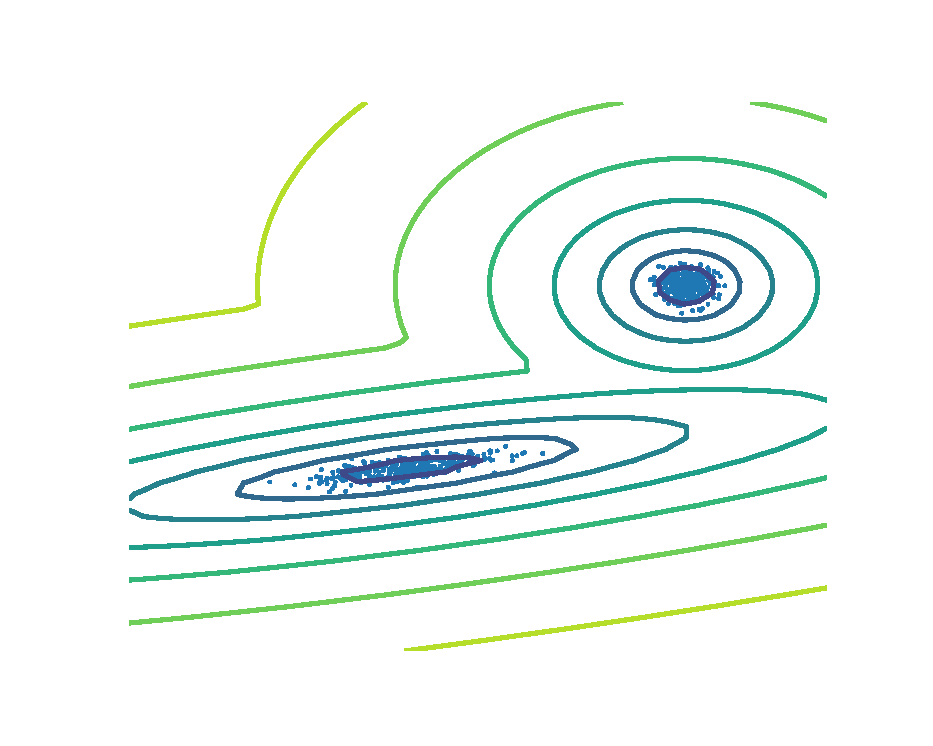
\includegraphics[width=0.33\textwidth]{figs/gmm.eps}
			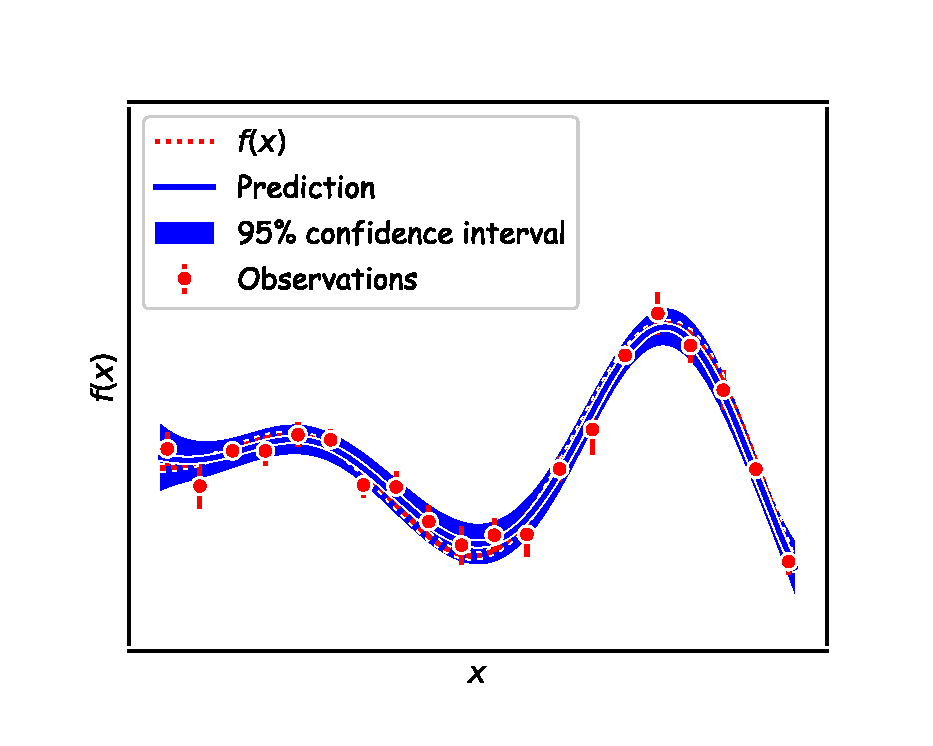
\includegraphics[width=0.33\textwidth]{figs/gp.eps}
		\end{center}
	\end{figure}
	\begin{center}
		$\pi(x, \theta)$~(joint probability) 
	\end{center}
	\begin{itemize}		
		\item $\blacktriangleright$ 
		Update beliefs about model parameters given data\\
		$\bm{\pi(\theta|x)} = \frac{\color{blue!50!green}{\overbrace{\pi(x|\theta)}^{\text{\clap{\textcolor{blue!50!green}{data likelihood~}}}}} \color{blue!70!red}{\overbrace{\pi(\theta)}^{\text{\textcolor{blue!70!red}{\clap{~prior}}}}}}{\color{blue}{\underbrace{\pi(x)}_{\text{\clap{\textcolor{blue}{evidence}}}}}}$~(Bayes' theorem)
		\item $\blacktriangleright$
		Compute predictive probabilities on unseen data
		$ \pi(x^\star| x) = \int \pi(x^\star |\theta)\color{black}{\bm{\pi(\theta|x)}} d\theta \approx \frac{1}{S} \sum_{s=1}^{S} \pi(x^\star|\theta_s)$, 
		$\theta_s \sim \pi(\theta|x)$, for $s=1\ldots S$
	\end{itemize}
\end{frame}


\begin{frame}
	\frametitle{Large Scale Inference}
	\begin{itemize}
		\item  $\circ$ Update beliefs given \textbf{massive-scale} data \includegraphics[width=2cm,height=2cm]{figs/Bayes.png} \hfill $\pi(\theta|x) = \frac{1}{Z} \pi(x|\theta) \pi(\theta)$ \hfill \textcolor{darkred}{Hard to compute!}
		\item  $\circ$ \textbf{Intuition:} For parametric models there is lot of \texbf{redundancy}---\textbf{\emph{compress the dataset}} into a summary and run inference thereon
	\end{itemize}
	\begin{figure}{\textwidth}
		\centering
		\includegraphics[width=7cm]{figs/coresets_high_level.png}
		\label{fig:coresets_high_level}
	\end{figure}
\end{frame}


\begin{frame}
	\frametitle{Problem Statement}
	\begin{tcolorbox}[colback=gray!5,colframe=white!40!black]  
		\centering
		\textbf{In modern ML, datasets scale outpaces our ability to process them}
	\end{tcolorbox}
	\textbf{Proposal: Replace datasets with \emph{coresets}} 
	\begin{itemize}
		\item $\blacktriangleright$ \texbf{\emph{scale up}} expensive inference methods
		\item $\blacktriangleright$ good \texbf{\emph{quality monitoring/statistical guarantees}}
		\item  $\blacktriangleright$ high degree of \texbf{\emph{automation}}, black-box inference
		\item $\blacktriangleright$ \texbf{\emph{general purpose}} Bayesian inference, for
	 \emph{conditionally independent data}, \emph{tractable likelihood functions} 
		\item  $\blacktriangleright$ \textbf{overall} good statistical/computational trade-off \emph{under statistical privacy and robustness constraints}
	\end{itemize}
\end{frame}

\begin{frame}
	\frametitle{Bayesian coresets at a glance: From importance sampling to variational inference}
	\begin{align*}
	\mcL(w, \theta):=\sum_{n=1}^{N} w_n \mcL_n(\theta), \;\;\text{s.t.}\;\; |\mcL(w, \theta) - \mcL(\theta)| \leq \eps |\mcL(\theta)|, \;\;\forall \theta \in \Theta
	\end{align*}
	$\blacktriangleright$ Principles of subset selection
	\begin{itemize}
		\item $\circ$ \textbf{Importance sampling} using \emph{sensitivity} $\sigma_n := \underset{\theta \in \Theta}{\sup}\big|\frac{\mcL_n(\theta)}{\mcL(\theta)}\big|$~\citep{huggins16}
		\item $\circ$ \textbf{Sparse regression} using \emph{inner product norms} $ \big\langle \mcL - \mcL(w), \mcL_n \big\rangle_\mcH$~\citep{campbell19jmlr}
		\item $\circ$ \textbf{Sparse variational inference} using the \emph{KL divergence} ~\citep{campbell19neurips}
	\end{itemize}
\end{frame}	

\begin{frame}
		\frametitle{Privacy}
		\begin{figure}
			\centering 
			\includegraphics[width=5cm,height=4cm]{figs/dp.png}
			\caption{Differential Privacy (DP) visually \emph{(\textsuperscript{\textcopyright}Aaron Roth)}}
		\end{figure}
	\textbf{Approximate DP}: A randomized mechanism $\mcM : X \rightarrow Y$ is $(\veps, \delta)$-DP if for \emph{\textbf{all}} neighbouring inputs $x, x': x \approx x'$ and \emph{\textbf{all}} sets of outputs $E \subseteq Y$ we have 
	$P[\mcM(x) \in E] \leq e^\veps P[\mcM(x') \in E] + \delta$
\end{frame}


\begin{frame}
	\frametitle{Robustness}
	Huber's $\eps$-contamination model
	\begin{columns}
		\begin{column}{.39\textwidth}
			\hfill \includegraphics[width=1.\textwidth]{figs/Huber.jpg}\\ 
		\end{column}
		\begin{column}{.69\textwidth}
			\hfill \includegraphics[width=.5\textwidth]{figs/contaminated-gaussian.png}\\ 
		\end{column}
	\end{columns}
	\definecolor{darkred}{rgb}{0.55, 0.0, 0.0}
	$(x_n)_{n=1}^{N}\sim G_{\eps, q}:= (1-\eps)\cdot \pi + \eps \cdot \color{darkred}{q}$~\citep{huber92},
	where
	\\  $\circ$ $\eps \in (0,1)$, 
	\\  $\circ$ $\pi$ follows our statistical assumptions, and 
	\\  $\circ$ $\color{darkred}{q}$ is an arbitrary distribution of outliers
\end{frame}


\begin{frame}
	\frametitle{Robustness}
	\begin{columns}
		\begin{column}{0.48\textwidth}
			\centering 
			\includegraphics[width=3.6cm,height=3.4cm]{figs/density.png}%
		\end{column}
		\begin{column}{0.48\textwidth}
			\centering
			\includegraphics[width=3.6cm,height=3.4cm]{figs/influence.png}%
		\end{column}
	\end{columns}
		\begin{itemize}
			\item $\blacktriangleright$ \textbf{Influence functions}: $IF(q, T, G) = \frac{\partial}{\partial \eps} T(G_{\eps, q}(x))\Bigg\rvert_{\eps=0}$ \citep{huber09}.
			\item $\blacktriangleright$ \textbf{Bayesian sensitivity}: metric between posteriors conditioned on neighboring datasets, e.g. $D_{FR}(\{x_i\}) \leftarrow \text{distance}(\pi(\theta|x)||\pi(\theta|x\cup\{x_i\}))$\citep{kurtek15}.	
		\end{itemize}
\end{frame}


\begin{frame}{Structure}
	\begin{itemize}
		\item[I.]\textbf{Bayesian Pseudocoresets} \small{\citep{psvi}} \\
		A variational framework for scalable Bayesian inference, that achieves superior summarization quality in high-dimensions and admits differentially private constructions
		\item[II.]\textbf{$\beta$-Cores} \small{\citep{beta-cores}}  \\
		A framework for Bayesian summarization designed for observations following the Huber contamination model.
	\end{itemize}
\end{frame}


%%%%%%%%%%%%%%%%%%%%%%%%%%%%%%%%%%%%%%%%%%%%%%%%%%%%%%%
%%%%%%%%%%%%%%%%%%%%%%%%%%%%%%%%%%%%%%%%%%%%%%%%%%%%%%%

%%%%%%%%%%%%%%%%%%%%%%%%%%%%%%%%%%%%%%%%%%%%%%%%%%%%%%%
%%%%%%%%%%%%%%%%%%%%%%%%%%%%%%%%%%%%%%%%%%%%%%%%%%%%%%%
%% NEURIPS
%%%%%%%%%%%%%%%%%%%%%%%%%%%%%%%%%%%%%%%%%%%%%%%%%%%%%%%
%%%%%%%%%%%%%%%%%%%%%%%%%%%%%%%%%%%%%%%%%%%%%%%%%%%%%%%

\begin{frame}
	\LARGE{\textbf{I. Bayesian Pseudocoresets}}
\end{frame}



\begin{frame}
	\frametitle{Bayesian Coresets}
	$\circ$ \textbf{Riemannian Coresets}~\citep{campbell19neurips}
	\begin{figure}
		\includegraphics[width=1.\linewidth]{figs/sparsevi_posterior.png}
	\end{figure}
	$\circ$ \textbf{Sparse Variational Inference}
	\begin{align*}
	 w^\star = \argmin_{w\in\reals^N} \kl{\pi_w}{\pi}\label{eq:coresets-vi} \quad \quad
	\text{s.t.} \quad w \geq 0, \; \|w\|_0 \leq M
	\end{align*}
\end{frame}

\begin{frame}
	\frametitle{Limitation I: High-dimensional data}
	\begin{tcolorbox}[colback=grey!5,colframe=white!40!black,title=KL lower bound in Gaussian mean inference via coresets]  
		\begin{itemize}
		\item $\circ$ Data $(X_n)_{n=1}^N \distiid \distNorm(0, I)$ in $\reals^d$, prior
		$\mu \dist \distNorm(0, I)$, likelihood
		$(X_n)_{n=1}^N  \distiid \distNorm(\mu, I)$
		\item  $\circ$ Coreset size $ M $, \emph{optimal} coreset posterior $\pi_{w^\star}$ 
		\item $\blacktriangleright$ Then $\forall M<d$ with high probability
		\begin{align*}
		\kl{\pi_{w^\star}}{\pi} \geq \frac{1}{2}\frac{N-M}{1+N} F(d-M, M, N)
		\end{align*}
		(RHS visualized in next slide)
		\end{itemize}
	\end{tcolorbox}
\end{frame}


\begin{frame}
	\frametitle{Limitation I: High-dimensional data}
			\centering
	\begin{figure*}
		\includegraphics[width=.8\linewidth]{figs/klbound.png}
	\end{figure*}
\end{frame}

\begin{frame}
	\frametitle{Limitation I: High-dimensional data}
	$\circ$ In Gaussian mean inference coreset covariance and mean are 
	\begin{align*}
	\Sigma_w &=\left(1+\sum_{n=1}^N w_n\right)^{-1} I, & \mu_w &= \Sigma_w \sum_{n=1}^N w_n X_n.\label{eq:gausswpost}
	\end{align*}
	
	which can be replicated via \emph{a point}
	\begin{align*}
	& U = \left(\sum_{n=1}^Nw_n\right)^{-1}\sum_{n=1}^N w_nX_n
	& \text{with weight}\;\; \sum_{n=1}^N w_n.
	\end{align*}
	$\circ$ True posterior can be exactly computed via a \textbf{\emph{single pseudopoint}}
	\begin{align*}
	& U = \frac{1}{N}\sum_{n=1}^N X_n & \text{with weight}\;\; N.
	\end{align*}
\end{frame}

\begin{frame}
	\frametitle{Limitation II: Privacy}
	\begin{itemize}
		\item $\circ$	Existing constructions are incompatible with formal privacy definitions, as subset
		of datapoints gets revealed 
		\item $\circ$	For sensitive datasets, summarization
		should use synthetic data
		\begin{figure*}
			\includegraphics[width=1\linewidth]{figs/dp_summarize.png}
		\end{figure*}
	\end{itemize}
\end{frame}

\begin{frame}
	\frametitle{Applications of summarization: (Pseudo)data as \emph{"approximate sufficient statistics"}}
	\begin{itemize}
		\item For scalability
		\begin{itemize}
			\item $\blacktriangleright$ Linear regression, clustering, herding, priors for DGMs~\citep{bachem15,bachem17}
			\item $\blacktriangleright$ Nystr\"{o}m method, leverage scores for computing with kernels~\citep{drineas05,musco17,agrawal19},
			\item $\blacktriangleright$ Inducing (pseudo-)input methods in Gaussian processes~\citep{snelson05,titsias09,bauer16}
		\end{itemize}
		\item For privacy
		\begin{itemize}
				\item $\blacktriangleright$ Kernel mean embeddings, sparse regression~\citep{zhou08,balog18}
		\end{itemize}
	\end{itemize}
\end{frame}

\begin{frame}
	\frametitle{Bayesian Pseudocoresets}
		\begin{itemize}
		\item  $\blacktriangleright$ Pseudocoreset posterior
	\begin{align*}
		\pi_{u,w}(\theta) = \frac{1}{Z(u, w)} \exp \left( \sum_{m=1}^{M} w_m f(u_m,\theta) \right) \pi_0(\theta)
	\end{align*}
	where $(u_m)_{m=1}^{M}$ are \textbf{learnable pseudodata points}.
		\item  $\blacktriangleright$ Variational inference over \textbf{pseudodata locations} and \texbf{weights}
	\begin{align*}
	u^\star, w^\star = \argmin_{\substack{u\in\reals^{d \times M}}, w\in\reals^M_+}\,\, \kl{\pi_{u,w}}{\pi}. 
	\end{align*}
		\end{itemize}
\end{frame}


\begin{frame}
	\frametitle{Pseudocoresets Construction}
	\begin{align*}
	u^\star, w^\star = \argmin_{\substack{u\in\reals^{d \times M}}, w\in\reals^M_+}\,\, \kl{\pi_{u,w}}{\pi}. 
	\end{align*}	
	 $\circ$ Gradients \wrt variational parameters are tractable 
	\begin{align*}
	\nabla_{u_m}\mathrm{D}_{\mathrm{KL}} = -w_m\cov_{u,w}\left[(\nabla_u f)(u_m), f(x, \theta)^T1 - f(u, \theta)^Tw\right]
	\end{align*}
	\begin{align*}
	 \nabla_w\mathrm{D}_{\mathrm{KL}} = - \cov_{u,w}[f(u, \theta) ,f(x, \theta)^T1 - f(u, \theta)^Tw]
	\end{align*}
\end{frame}


\begin{frame}
	\frametitle{Black-box Batch  Pseudocoreset Construction}
	\vspace{-0.5cm}
	\begin{itemize}
		\item $\blacktriangleright$ Pseudocode sketch
		\scriptsize 
		\begin{tcolorbox}
			\begin{algorithmic}[1]
				\Procedure{PSVI}{ likelihood function $f$, data $x$, prior $\pi_0$, coreset size $M$, minibatch size $B$, $\#$ of optimization steps $T$, $\#$ of samples from coreset iterates $S$, learning rate schedule $(\gamma_t)_{t=0}^{\infty}$}
				\LineCommentIndent{\textbf{Initialize} using a uniformly chosen subset of the full dataset}
				\For{$ t = 1, \ldots, T$} 
					\LineCommentIndent{\mbox{Take $S$ samples from current pseudocoreset posterior}}\\
					\LineCommentIndent{\mbox{Get a minibatch of $B$ points from the full dataset}} 
						\For{$s = 1, \dots, S$} 	
							\LineCommentIndent{\mbox{Compute (gradient) log-likelihood discretizations}}\\
						\EndFor
					\LineCommentIndent{\mbox{Take steps using MC \textbf{gradients for $w$ and $u$}}}
				\EndFor
				\State\Return $w$, $u$%, $\beta$
				\EndProcedure		 
			\end{algorithmic}
		\end{tcolorbox}
		\normalsize
	\end{itemize}
\end{frame}

\begin{frame}
	\frametitle{Differentially Private Construction of Bayesian Pseudocoreset}
	\vspace{-4pt}
	\begin{columns}
		\begin{column}[t]{0.4\textwidth}
		\begin{itemize}
			\item $\blacktriangleright$ \textbf{Initialize}  from the statistical model
			\item $\blacktriangleright$ \textbf{Iterate} Compute private gradients via applications of the \textbf{subsampled Gaussian mechanism}~\citep{abadi16}
		\end{itemize}
		\end{column}
	\pause
		\begin{column}[t]{0.6\textwidth}
		\begin{itemize}
			\item --- {Moments accountant}
			\item --- {No extra  cost when sampling from the coreset}
			\item --- {No global sensitivity computation}
			\item --- {Adaptive gradient clipping} 
			\item --- {Constructed private pseudocoresets can be queried \emph{ad infinitum}} 
		\end{itemize}
		\end{column}
	\end{columns}
\end{frame}

\begin{frame}
	\frametitle{Experiments I~(High-dimensional Gaussian mean inference)}
	\centering 
	$\circ$ 500 dimensions, 1K datapoints\\
	\includegraphics[width=.49\textwidth]{figs/d500_pts_combined.png}
	\includegraphics[width=.49\textwidth]{figs/d500_KLDvsCstSize.png}
\end{frame}

\begin{frame}
	\frametitle{Experiments II~(Bayesian Linear Regression)}
	\centering
	\begin{columns}
		\begin{column}{.5\textwidth}
		$\circ$ Synthetic dataset
		\\---101 dimensions,
		\\---2K datapoints
		\end{column}
		\begin{column}{.5\textwidth}
		\includegraphics[width=1.\textwidth]{figs/linregKLDvsCstSize.png}
		\end{column}
	\end{columns}
\end{frame}

\begin{frame}
	\frametitle{Experiments III~(Bayesian Logistic Regression)}
	\centering 
	$\circ$ 2-237 dimensions, 500-100K datapoints\\
	\includegraphics[width=.3\textwidth]{figs/wsanta100K_KLDvssz.png}
	\includegraphics[width=.3\textwidth]{figs/wds1100_KLDvssz.png}
	\includegraphics[width=.3\textwidth]{figs/fma_KLDvscput.png} \\
	\includegraphics[width=.3\textwidth]{figs/wsanta100K_privacy.png}
	\includegraphics[width=.3\textwidth]{figs/wds1100_privacy.png}
	\includegraphics[width=.3\textwidth]{figs/wfma_privacy.png} 
	\small $\delta=\frac{1}{N}$
	\normalsize
\end{frame}




%%%%%%%%%%%%%%%%%%%%%%%%%%%%%%%%%%%%%%%%%%%%%%%%%%%%%%%
%%%%%%%%%%%%%%%%%%%%%%%%%%%%%%%%%%%%%%%%%%%%%%%%%%%%%%%
%% WSDM
%%%%%%%%%%%%%%%%%%%%%%%%%%%%%%%%%%%%%%%%%%%%%%%%%%%%%%%
%%%%%%%%%%%%%%%%%%%%%%%%%%%%%%%%%%%%%%%%%%%%%%%%%%%%%%%


\begin{frame}
	\LARGE{\textbf{II. $\beta$-Cores: Robust large-scale Bayesian data summarization in the presence of outliers}}
\end{frame}





\begin{frame}[fragile,t]
	\frametitle{Challenges}
	\begin{columns}[onlytextwidth]
		\begin{column}{0.35\textwidth}  %%<--- here
			\vspace{-1cm} 
			
			\begin{center}
				\begin{figure}
					\includegraphics[width=0.9\textwidth,angle=5]{figs/crowds.jpg}
				\end{figure}
				
				\vspace{-.35cm} 
				
				\begin{figure}
					\includegraphics[width=0.9\textwidth,angle=-5]{figs/Four-No-Three.jpg}
					\caption*{The Hierarchy of Disagreement by Paul Graham}
				\end{figure}
				
				\vspace{-.35cm} 
				
				\begin{figure}
					\includegraphics[width=0.9\textwidth,angle=-5]{figs/spam.jpg}
				\end{figure}
			\end{center}
		\end{column}
		\begin{column}{0.65\textwidth}
			\vspace{-2.6cm} 
			
			\begin{itemize}
				\item $\blacktriangleright$ Web-scale ML systems on \emph{\textbf{massive}} data from \emph{\textbf{multiple sources}}
				\item $\blacktriangleright$ \textbf{Requirement 1}: \emph{Scalability}  via reducing redundancy
				\item $\blacktriangleright$ \textbf{Requirement 2}: \emph{Robustness to statistical misspecification} caused by observations, and/or model assumptions   
				\item $\blacktriangleright$ \textbf{$\beta$-Cores}: summarizations robust to contamination as an \textbf{integrated approach to data cleaning \emph{and} scalable inference} with high automation
			\end{itemize}
		\end{column}
	\end{columns}
\end{frame}

\begin{frame}
	\frametitle{Background}
	$\blacktriangleright$ \textbf{Outliers} are typically 
	\begin{itemize}
		\item $\circ$ treated \textcolor{blue}{separately from inference}, and
		\item $\circ$ tackled via \textcolor{blue}{computing distances} within datapoints~\citep{diakonikolas19, dickens20}, or
		\item $\circ$ introducing \textcolor{blue}{data redudancies}~\citep{raykar10, karger11}.
	\end{itemize} 
	\pause
	$\blacktriangleright$ Such approaches \emph{\textbf{scale adversely}} with data \textbf{dimensionality} and \textbf{size}, often decreasing automation or imposing assumptions on outliers.
\end{frame}

\begin{frame}
	\frametitle{Background}
	$\blacktriangleright$ \textbf{Robustified Bayesian inference} via 
	\begin{itemize}
		\item --- \textcolor{blue}{heavy-tailed data likelihood functions}~\citep{huber09, insua12}
		\item --- \textcolor{blue}{localization}~\citep{definetti61, wang18}
		\item --- \textcolor{blue}{data reweighting}~\citep{wang17} 
		\item --- \textcolor{blue}{robust gradient estimates in MC methods}~\citep{bhatia19}
		\item --- \textcolor{blue}{pseudo-Bayesian posteriors with reduced sensitivity}: robust divergences, coarsening~\citep{futami18, knoblauch18, miller19}
	\end{itemize}
	\begin{figure}
		\begin{center}
			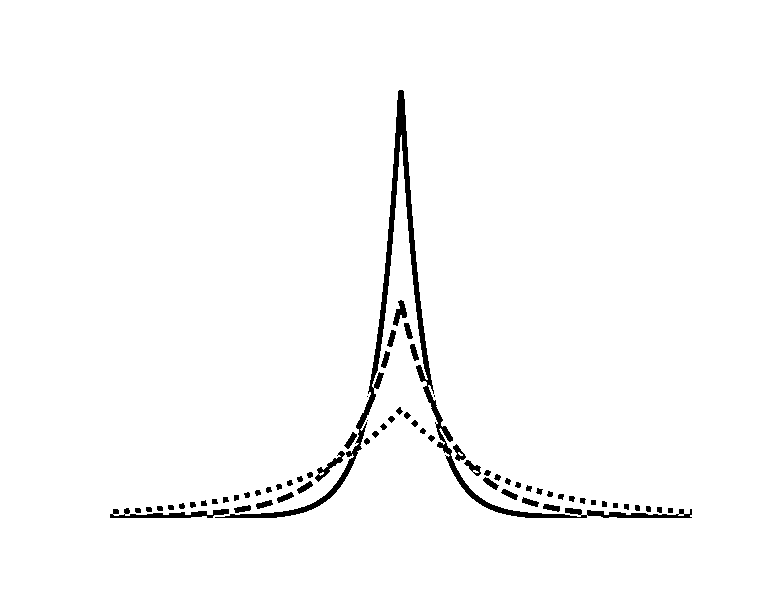
\includegraphics[width=0.24\textwidth,valign=c]{figs/heavy_tails.eps}
			\includegraphics[width=0.24\textwidth,valign=c]{figs/original.png}
			\includegraphics[width=0.24\textwidth,valign=c]{figs/localized.png}
			\includegraphics[width=0.24\textwidth,valign=c]{figs/reweighted.png}
		\end{center}
	\end{figure}
	\qquad heavy-tails \qquad\qquad \qquad\qquad\quad localization \qquad reweighting
	
\end{frame}




\begin{frame}
	\frametitle{Bayes' theorem: An optimization perspective}
	\centering 
	\begin{columns}
		\begin{column}{.79\textwidth}
			Bayes' rule as an optimization problem~\citep{zellner88}
		\end{column}
		\begin{column}{.29\textwidth}
			\hfill \includegraphics[width=1.\textwidth]{figs/Zellner.jpg}\\ 
		\end{column}
	\end{columns}
	\begin{equation*}
	\arg \underset{q(\theta) \in \mcP}{\min}  \left(\kl{q(\theta)}{\pi_0(\theta)} + \bm{N}\EE_{q(\theta)}\left[\kl{\hpi(x)}{\pi(x|\theta)}\right]\right),
	\end{equation*}
	giving
	\begin{align*}
	\pi(\theta|x) = \frac{1}{Z'} \exp\left(-\xent{\hpi(x)}{\pi(x|\theta)}\right)\pi_0(\theta),
	\end{align*}
	where $\hpi(x):=\frac{1}{N}\sum_{n=1}^{N}\delta(x-x_n)$ and $\xent{\hpi(x)}{\pi(x|\theta)}:=-\sum_{n=1}^{N}\log\pi(x_n|\theta)$~(cross-entropy).\\
	\emph{"Cost"} of the observations \emph{under the KL divergence}. 
\end{frame}


\begin{frame}
	\frametitle{Generalized Bayesian inference via $\beta$-divergence}
	$\blacktriangleright$ \textbf{Replace the KL} with the \emph{$\beta$- or density power divergence}~\citep{basu98}.
	\begin{align*}
	\arg \underset{q(\theta) \in \mcP}{\min}  \left(\kl{q(\theta)}{\pi_0(\theta)} + \bm{N}\EE_{q(\theta)}\left[\db{\hpi(x)}{\pi(x|\theta)}\right]\right),
	\end{align*}
	$\blacktriangleright$ \textbf{$\beta$-posterior}~\citep{futami18}:
	\begin{align*}
	\pi_\beta(\theta|x) \propto \exp\left(-\db{\hpi(x)}{\pi(x|\theta)}\right)\pi_0(\theta),
	\end{align*}
	where \\
	$\db{\hpi(x)}{\pi(x|\theta)} := -\sum_{n=1}^{N}  \underbrace{\left(\frac{\beta+1}{\beta}\pi(x_n|\theta)^{\beta} + \int_{\mcX} \pi(\chi|\theta)^{1+\beta}d\chi\right)}_{:=f_n(\theta)}$, with $\beta>0$.
\end{frame}


\begin{frame}
	\frametitle{Generalized Bayesian inference via $\beta$-divergence}
		$\db{\hpi(x)}{\pi(x|\theta)} := -\sum_{n=1}^{N}  \underbrace{\left(\frac{\beta+1}{\beta}\pi(x_n|\theta)^{\beta} + \int_{\mcX} \pi(\chi|\theta)^{1+\beta}d\chi\right)}_{:=f_n(\theta)}$, with $\beta>0$.
	\begin{itemize}
		\item $\circ$ \emph{\textbf{solves robustness}}: different strengths of influence to each datapoint, downweighting outliers \cmark
		\item $\circ$ when $\beta \rightarrow 0$ \emph{\textbf{classical}} Bayesian posterior gets recovered
		\item $\circ$ \emph{\textbf{still difficult to compute}}:~same scalability issues with classical Bayesian posterior \color{red}{\xmark}
	\end{itemize}
\end{frame}

\begin{frame}
	\frametitle{Coresets for $\beta$-posterior}
	$\blacktriangleright$  \textbf{Sparse $\beta$-posterior}
	\begin{align*}
	\pi_{\beta,w}(\theta|x) 
	:= \frac{1}{Z(\beta, w)}  \exp\left(\sum_{n=1}^{N}w_nf_n(\theta)\right)\pi_0(\theta)
	\end{align*}
	$\blacktriangleright$  Variational formulation
	\begin{align*}
	w^{*} = \arg \min_{w\in\reals^{N}} \kl{\pi_{\beta,w}}{\pi_{\beta}} 
	\quad
	\text{s.t.}
	\quad
	w \geq 0,\; ||w||_0 \leq M.
	\end{align*}
	$\blacktriangleright$  Analytical gradients~\citep{campbell19neurips}
	\begin{align*}
	\nabla_{w}\kl{\pi_{\beta,w}}{\pi_\beta} 
	& = -\cov_{\beta,w}\left[f,(1 -w)^Tf\right],
	\end{align*}
	where $f:=\left[f_1(\theta) \ldots f_N(\theta)\right]^T$.
\end{frame}

\begin{frame}
	\frametitle{Optimization scheme}
	\begin{align*}
	\text{For } & m=1,\ldots,M\\
	&\text{(1)~Next datapoint selection~(\emph{Discrete optimization})} \\
	&m^\star = \underset{m\in[N]}{\argmin} \kl{\pi_{\beta, w \leftarrow w \cup \{x_m\}}}{\pi_\beta}\\
	&\text{(2)~Coreset reweighting~(\emph{Continuous optimization})}\\
	&w^\star = \underset{w \in \reals^{N}_{\geq 0}}{\argmin}\kl{\pi_{\beta, w}}{\pi_\beta}\\ 
	\end{align*}
\end{frame}


\begin{frame}
		\frametitle{Next datapoint selection}
		\begin{itemize}
			\item ---Ideally: select greedily, via maximizing locally the decrease in KL (\emph{ignoring the effects of reweighting step})
			\item ---Sample from all possible expansions: likely \emph{negligible effects}
			\item ---Generally objective is \emph{non-submodular}
			\item $\circ$ \textbf{Solution}: \emph{Maximize correlation} with residual error 
		\end{itemize}
		\begin{center}
		\includegraphics[width=5cm,height=3cm]{figs/next-point-selection.png}\\
		\end{center}
	$\blacktriangleright$ Works seamlessly when summarizing batches
\end{frame}


\begin{frame}
	\frametitle{2-step black-box incremental sparse approximation of the $\beta$-posterior}
	\begin{itemize}
		\item $\blacktriangleright$ Pseudocode sketch
		\scriptsize 
		\begin{tcolorbox}
			\begin{algorithmic}[1]
				\Procedure{\bcore}{$\beta$, likelihood function, coreset size $M$, minibatch size $B$, $\#$ of optimization steps $T$, $\#$ of samples from coreset iterates $S$}
				\LineCommentIndent{ \textbf{Initialize} from the prior}			 
				\For{$\text{coreset size~}m =1, \ldots, M $}
				\LineCommentIndent{Get $S$ samples from coreset posterior}\\
				\LineCommentIndent{\textbf{Select next coreset point} via max-correlation with residual error computed on a random minibatch from the full dataset}			 
				\For{$ t = 1, \ldots, T$}
				\LineCommentIndent{Get $S$ samples from coreset posterior}
				\LineCommentIndent{\textbf{Reweight} via Monte-Carlo gradient descent}
				\EndFor
				\EndFor
				\State\Return $w$%, $\beta$
				\EndProcedure		 
			\end{algorithmic}
		\end{tcolorbox}
		\normalsize
		\pause 
		\item $\blacktriangleright$ Computational complexity $O(M(M+B)ST)$
	\end{itemize}
\end{frame}

\begin{frame}
	\frametitle{Experiment I: Gaussian Mean Inference under Stuctured Data Contamination}
	\centering
	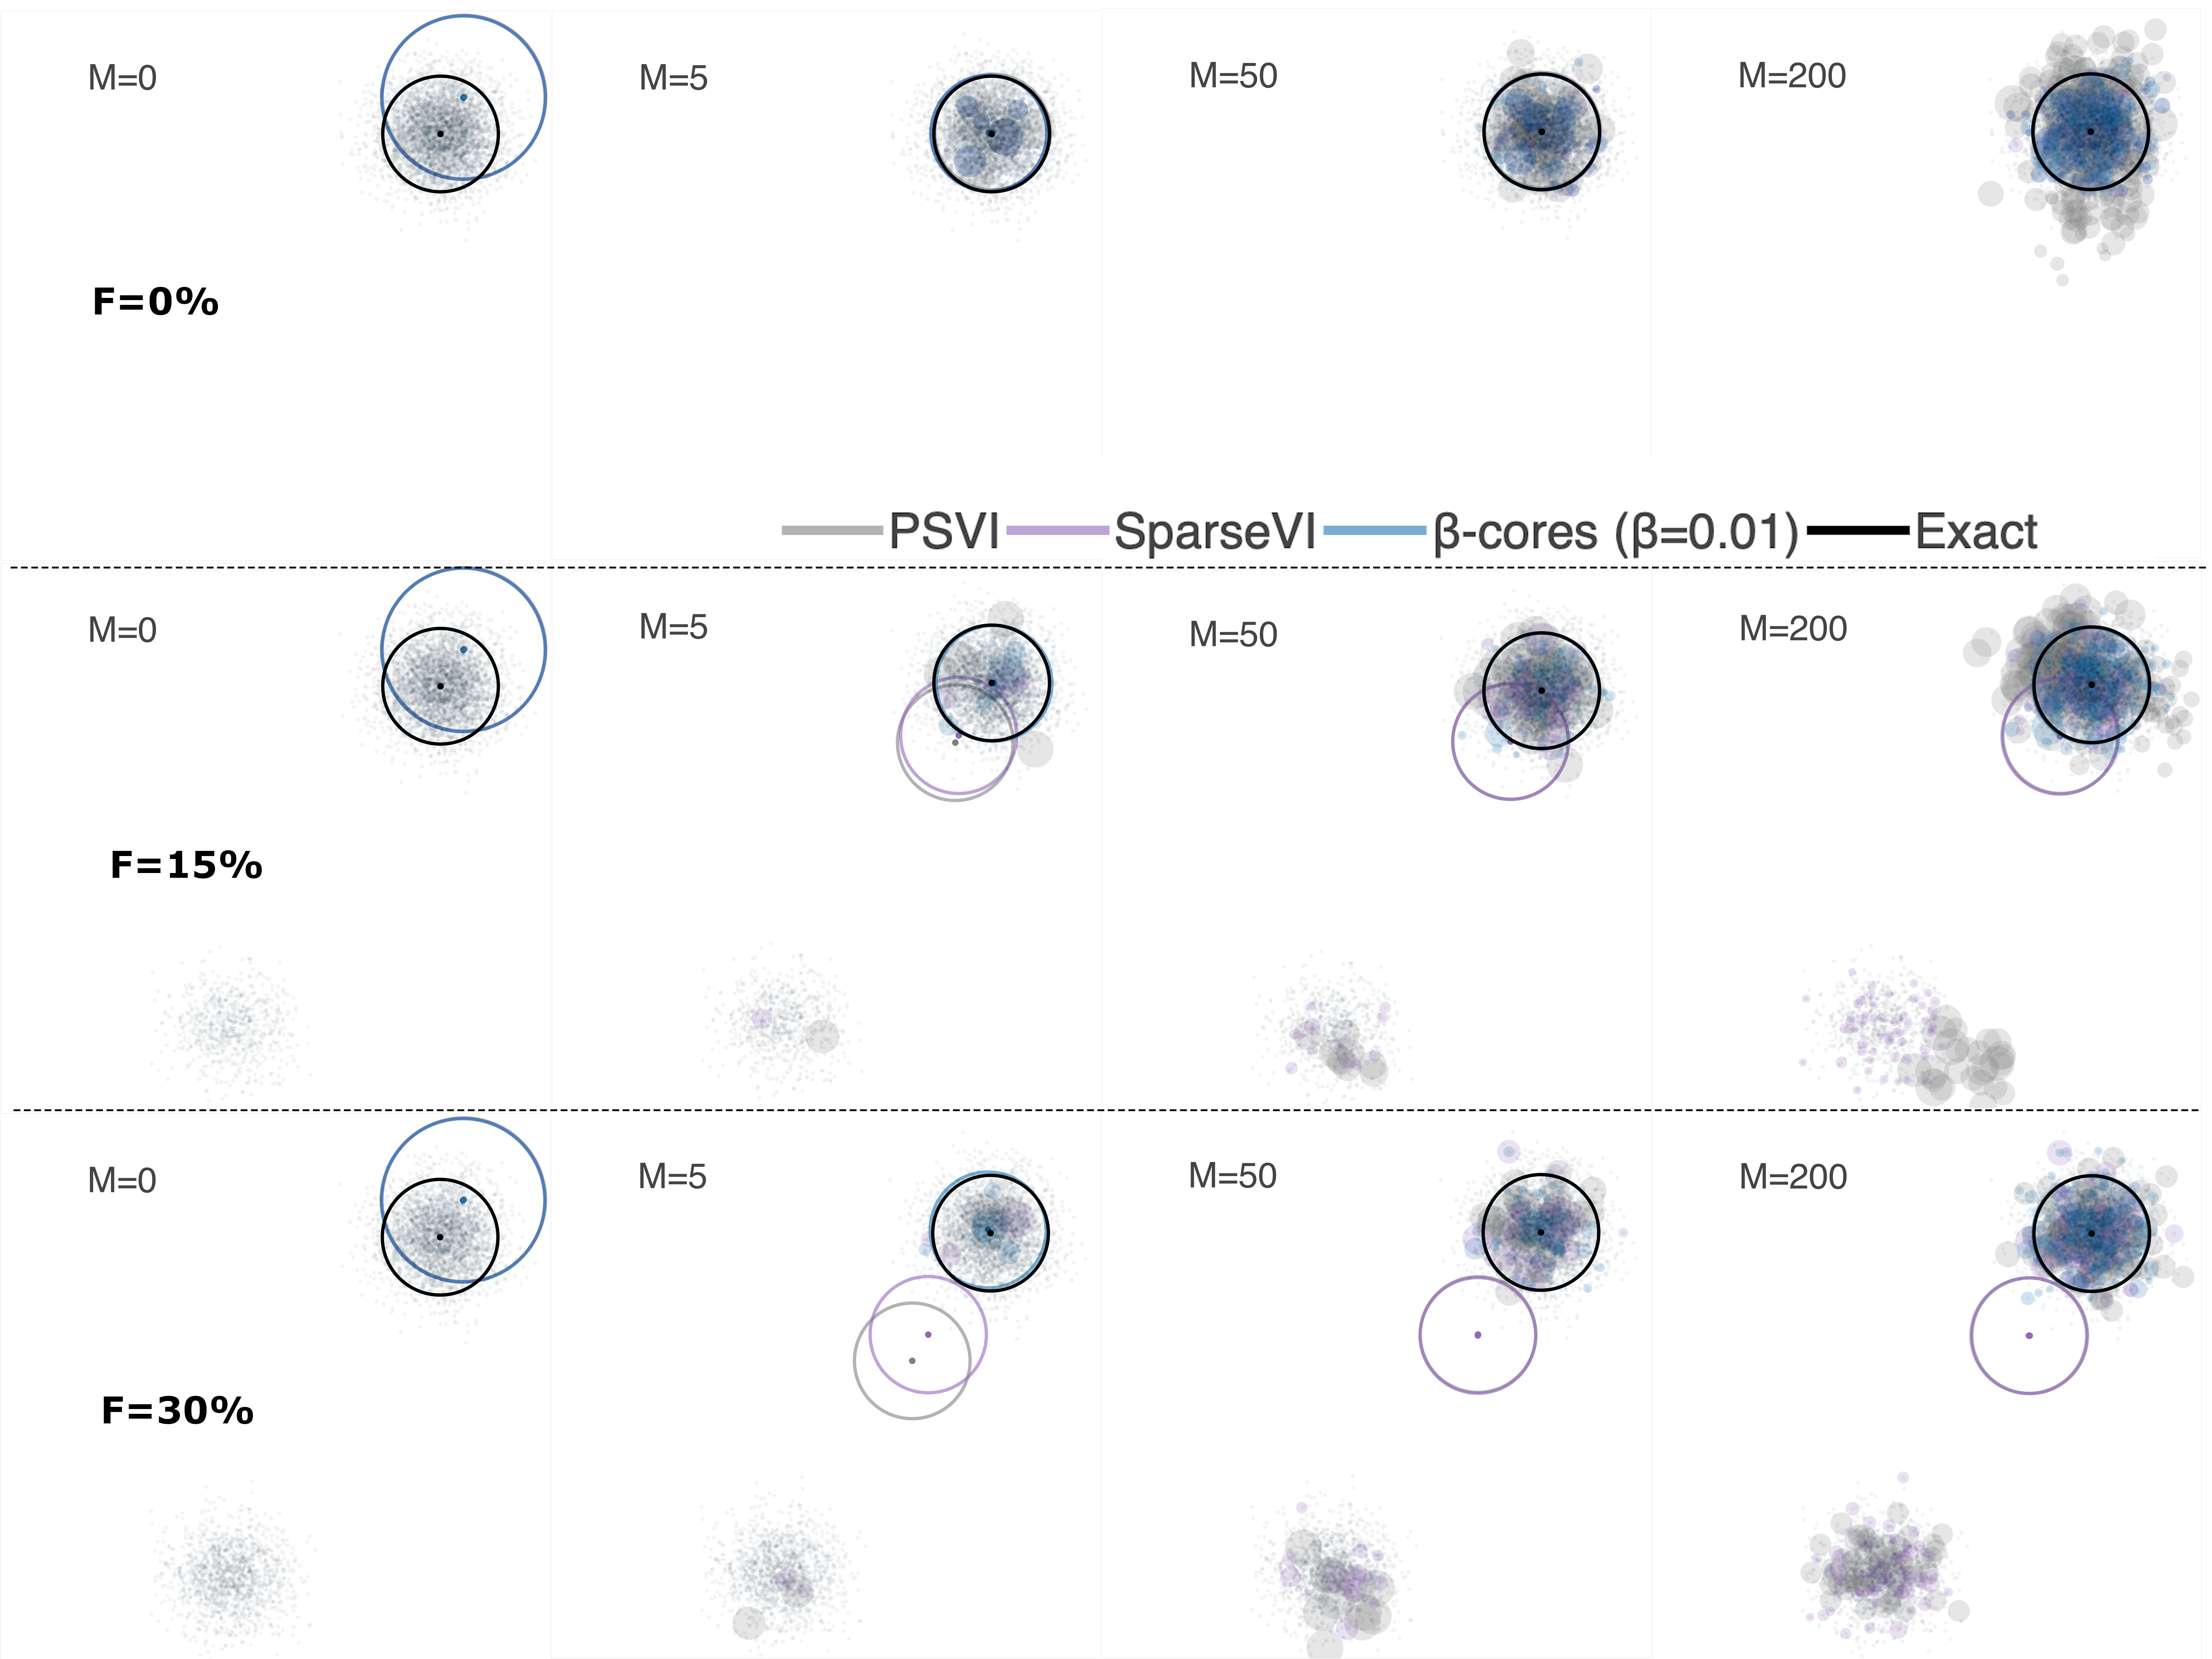
\includegraphics[width=.63\textwidth, height=4.35cm]{figs/gauss_scatterplot.png}\\
	\includegraphics[width=.3\textwidth]{figs/f0KLDvsCstSize.png}
	\includegraphics[width=.3\textwidth]{figs/f15KLDvsCstSize.png}
	\includegraphics[width=.3\textwidth]{figs/f30KLDvsCstSize.png}
\end{frame}

\begin{frame}
	\frametitle{Gaussian Mean Inference under Stuctured Data Contamination: Effects of varying the robustness hyperparameter}
	\centering
			\centering
	\includegraphics[width=.325\textwidth]{figs/comp_beta_F0_KLDvsCstSize.png}
	\centering
	\hfill
	\includegraphics[width=.325\textwidth]{figs/comp_beta_F15_KLDvsCstSize.png}
	\centering
	\hfill
	\includegraphics[width=.325\textwidth]{figs/comp_beta_F30_KLDvsCstSize.png}
	\centering

\end{frame}

\begin{frame}
	\frametitle{Experiment II: Bayesian Logistic Regression under Mislabeling and Feature Noise}
	\centering
	\includegraphics[width=.49\textwidth, height=3.8cm]{figs/phish09_10_15_False_False_ACCvssz.png}
	\includegraphics[width=.49\textwidth, height=3.8cm]{figs/webspam09_10_15_True_False_ACCvssz.png}
	\includegraphics[width=.49\textwidth, height=3.8cm]{figs/phish07_10_0_False_False_ACCvssz.png}
	\includegraphics[width=.49\textwidth, height=3.8cm]{figs/webspam09_10_0_True_False_ACCvssz.png}
\end{frame}

\begin{frame}
	\frametitle{Experiment III: Neural Linear Regression on Noisy Data Batches}
	\centering
	\includegraphics[width=.49\textwidth, height=3.8cm]{figs/boston02_01_30_RMSEvssz.png}
	\includegraphics[width=.49\textwidth, height=3.8cm]{figs/year02_01_30_RMSEvssz.png}
	\includegraphics[width=.49\textwidth, height=3.8cm]{figs/boston02_01_0_RMSEvssz.png}
	\includegraphics[width=.49\textwidth, height=3.8cm]{figs/year02_01_0_RMSEvssz.png}
\end{frame}

\begin{frame}
	\frametitle{Experiment IV:  Subpopulations Selection for Budgeted Inference on Hospital Readmissions}
	\centering
	\includegraphics[width=.49\textwidth, height=3.8cm]{figs/group_diabetes06_10_01_False_ACCvsit.png}
	\includegraphics[width=.49\textwidth, height=3.8cm]{figs/group_diabetes06_10_01_False_ACCvssz.png}
	\includegraphics[width=.49\textwidth, height=3.8cm]{figs/group_diabetes06_10_0_False_ACCvsit.png}
	\includegraphics[width=.49\textwidth, height=3.8cm]{figs/group_diabetes06_10_0_False_ACCvssz.png}	
\end{frame}

\begin{frame}
	\frametitle{Experiment IV: Infomative Subpopulation Combinations for Budgeted Inference on Diabetes Patients' Readmissions}
	\centering
	\includegraphics[width=.49\textwidth]{figs/selected_groups.png}	
	\begin{itemize}
		\item $\blacktriangleright$ Older age Caucasian/Afro-American female group population is most informative ~\citep{ghorbani19}
		\item $\blacktriangleright$ More effective selection compared to data Shapley~\citep{shapley53}
	\end{itemize}
\end{frame}


\begin{frame}
	\frametitle{Conclusions}
	\centering
	We introduced a \\ \textbf{general-purpose  black-box} \\ Variational Inference method that \pause
	\begin{itemize}
		\item $\blacktriangleright$ addresses jointly \emph{\textbf{scalability and robustness to misspecification}} in  large-scale real-world ML applications
		\item $\blacktriangleright$ \emph{\textbf{maintains the strengths of Bayesian inference}}
		\item $\blacktriangleright$ \emph{\textbf{minimizes assumptions}} about the \emph{\textbf{model}} and the \emph{\textbf{outliers}}, and maintaining high automation
		\item $\blacktriangleright$ \emph{\textbf{preprocessing step}} compatible with black-box inference
		\item $\blacktriangleright$ points to an \emph{\textbf{efficient large-scale data subpopulations acquisition}}
	\end{itemize}
\end{frame}

\begin{frame}
	\frametitle{\textbf{Thank you!}}
	\centering
	\large{\textbf{Papers}}:\\ {https://proceedings.neurips.cc/paper/2020/\\file/ab452534c5ce28c4fbb0e102d4a4fb2e-Paper.pdf}\\{https://arxiv.org/abs/2008.13600}\\
	\vspace{1cm}
	\includegraphics[width=3.6cm,height=1.8cm]{figs/github-logo.png}\\
	\texttt{https://github.com/trevorcampbell/\\pseudocoresets-experiments}\\ \texttt{https://github.com/dionman/beta-cores}
\end{frame}


\begin{frame}[allowframebreaks]{References}
	\tiny %\scriptsize
	\bibliography{references.bib}
\end{frame}

\end{document}
